%!TEX root = ../../Main.tex
\graphicspath{{Chapters/Diskussion/}}
%-------------------------------------------------------------------------------


\section{Diskussion}
Igennem processen i projektet, mødte gruppen flere problemstillinger. Noget af det første var, at bestemme hvilket filter der skulle bruges for at løse opgaven. Efter søgen på nettet og gennem undervisningsbogen, blev et LMS filter valgt som den rette løsning. Hertil er der blevet produceret et filter, som er testet både i Matlab som simulering, og på blackfin processoren som realisering. 

Igennem testen oplevede gruppen flere forskellige problemstillinger som vil redegøres for herunder. 

\begin{description}[align=left]
\item [Første sample = 1.] Igennem testen blev den første sample sat til 1 i crosscore koden, dette gøres for at få det samme signal fra input til output. Dette betyder at fejlen allerede på første sample er stor, mens hvis første sample er 0, vil filteret lige så stille og roligt få en større fejl, og derved have en indjusteringstid. Derfor giver det bedre mening at bruge en værdi på 1. Dog ser vi en at fejlen e(n) forværes hvis den første værdi i matlab koden er 1 og ikke 0. Vi har ikke nogen god forklaring på hvorfor dette er tilfældet, vi mener dog at første værdi burde være 1 for at sende det samme signal igennem. 
\item [Filter koefficienter] har stor betydning for filteret, især når vi kigger på matlab koden. For at filtrere ordentlig på de forskellige toner og food processeren, skal filteret have 256 filter koefficienter i matlab. Modsat høres væsentlig forskel på blackfin, når vi kommer over 32 koefficienter, hvor den omtalte "klik" lyd forværes, hvis vi kommer på 64 eller derover. Vi har dog ikke nogen forklaring på hvorfor matlab modellen ikke kan filtrere støjsignalerne fra ved lav filter koefficienter. Det burde være muligt at filtrere helt ned til blackfin implementeringen, især hvis man tester med 3 rene sinus toner.   
\item [Simulering af realiseringen.] 
Da der blev simuleret det eksakte som vi realiserede på blackfin, var resultaterne  ikke hvad vi forventede (figur\ref{fig:Tjek_af_frek}), da det ikke ligner at funktionen e(n) = d(n) - y(n) bliver gennemført ordentlig. Hvis man kigger på skaleringen burde filteret trække støj tonerne fra det oprindelige signal. Den bedste forklaring vi havde på dette var at der bliver brugt for lidt koefficienter, så filteret ikke lavede et filter peak på den rigtige frekvens. Dette tjekkede vi dog i matlab, og fandt at de var ens, derfor kunne den teori afvises. 
På figur \ref{fig:filter_matlab}, ser vi filteret som bliver skab i matlab, og kan derved også se at filteret ikke filtrerer de frekvenser vi regner med. Dette filter er derfor ubrugeligt. 
\begin{figure}[H]
	\centering
	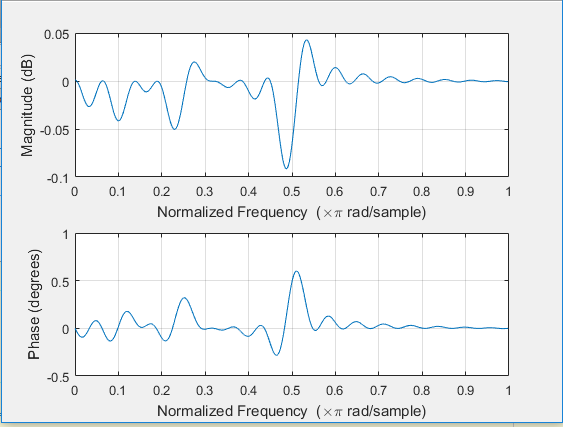
\includegraphics[width = 400pt]{Img/filter_matlab}
	\caption{Simulerings Filter af realiseringen i matlab}
	\label{fig:filter_matlab}
\end{figure}
\item [Food processor realisering] Da vi skulle teste om vores filter kunne filtrere på et mere komplekst signal end tre toner, har vi valgt at bruge en foodprocessor. Støjen fra foodprocessoren indeholder mange forskellige frekvenser, hvilket gør kravene til filteret højere. Da vi er begrænset til kun at have 32 koefficienter, begrænser det også, hvor mange frekvenser i støjsignalet, der kan dæmpes. Dette er en af grundene til at filteret ikke har haft den ønsket effekt. 
En anden grund kan også være at vores timing ikke har været god nok mellem støj signalet og tale-signalet. Da vi testede med enkelte toner fandt vi ud af at bare en lille ændring i støjsignalets frekvens gjorde filteret betydeligt dårligere til at dæmpe støjen. Så hvis timingen ikke har været præcis nok, har de forskellige frekvenser for støjsignalet ikke passet med støjen på talesignalet.
\item ["klik" lyde.] Som tidligere beskrevet opleves der "klik" lyde når filteret køres på blackfin. Den eneste gode forklaring vi har på dette, er at filterkoefficienterne ændres så hurtigt at de 'ødelægger' lyden med "klik" lyde. 
\item [Bedst udenfor 300-3400 Hz.] Vi fandt også ud af gennem projektet at LMS filteret fungerer bedst hvis det støjende signal (x(n)) og det ønskede signal (e(n)) ligger i forskellige frekvenser. Dette ses af figur \ref{fig:Filter_food}, hvor vi har et tale signal, som normalt ligger imellem 300-3400 Hz, sammensat af et food processor som støjer på et meget bredt spektrum. Det ses at filteret skaber et gain af støjen som er hensigten, når vi kommer over 3400 Hz. Dette betyder også at filteret kommer til at filtrere talesignalet, da de ligger inden for samme frekvensbånd. Dog har vi gennem projektet set at en ren sinus tone, godt kan filtreres fra selvom den ligger inderfor tale båndet. Dette skyldes højst sandsanligt at tonen er så kraftig at filteret negligere talesignalet. \\
Hvis der var uendelig processorkraft, kunne vi måske bruge krydskorralation, lave et krydskorralation på hver frekvens med støjen og derved finde peak hvor signalet og støjen korrelerer. Dette er dog ikke muligt på blackfin, da det vil bruge meget processorkraft, og memory, da hele støjsignalet ville skulle "krydses" med hele det oprindelige signal, for hver sample. 
\item [Ikke-funktionelle krav.]
\item [Løsning i sidste time.] Da vi stort set var færdige med rapport og kode, fandt vi en fejl i blackfin implementeringen, som forklarede og løste problemet med "klik" lydene som tidligere nævnt. 
Vi så ikke fejlen, når vi blot testede med 1024, da fejlen ligger når vi tage 2,3,4.... blok af 1024 samples. Dette betyder at at vi i den tidligere kode negligerede de første 32 samples, pga funktionens if løkker. I den nye implementering, har vi derved oprettet en ny buffer som gemmer de gamle koefficienter, så de kan bruges når en ny blok af 1024 samples kommer til det første loop. Vi sikre af vi peger det rigtige sted i bufferen, ved at sikre at hvis idxNew komemr under 0, sætter vi idxNew til NUM\_WEIGTHS-1 for at flippe pege pointeren op til det forrige værdi for filteret. Den nye kode kan ses herunder. Dette er en udkast til implementering, og derfor skal der også sættes tid af til at optimere koden. Vi testede herefter og fandt at "klik" lydene forsvandt. \\
\begin{lstlisting}
for(short i = 0; i < len; i++)
	{

		delay[idx] = x[i];
		idxNew = idx;
		if (++idx >= NUM_WEIGTHS) idx = 0;

		long fract yn = 0;

		for(short j = 0; j < NUM_WEIGTHS; j++)
		{
			//if(i > j)
			//{
				yn = yn + Filter.W[j]*delay[idxNew];
				if (--idxNew < 0) idxNew = NUM_WEIGTHS-1;
			//}
		}
		y[i] = (fract)yn;
		e[i] = d[i] - yn;

		long fract tmp_W = 0;

		for(short k = 0; k < NUM_WEIGTHS; k++)
		{
			if(i > k)
			{
				Filter.W[k] = Filter.W[k]  + my*x[i-k]*e[i];

			}
		}
	}
\end{lstlisting}

\item [Læringsmål.] Projektet er opbygget og leder kraftig op til læringsmålene for faget. Igennem dette projekt har vi derved undersøgt og arbejdet med hardware arkitektturen på DSP'en, dette vises og forklares gennem Struktur afsnittet. En real tids konfiguration er blevet lavet og testet gennem dette projekt, og endda til en vis grad opfyldt real tids implementeringen. Herunderover har vi udviklet og gennemarbejdet et filter som gør brug af en algoritme, herigennem LMS algoritmen, som kan ses under Teori afsnittet. Vi har ikke set meget på strømforbruget og optimering igennem dette projekt, da det ikke har været det essentielle for lige præcis dette projekt. Det vil dog kunne tages op ved efterarbejde.    


\end{description}

